%%% machine_learning_p2.tex
%%%
%%% This LaTeX source document can be used as the basis for your technical
%%% paper or abstract. Intentionally stripped of annotation, the parameters
%%% and commands should be adjusted for your particular paper - title, 
%%% author, article DOI, etc.
%%% The accompanying ``template.annotated.tex'' provides copious annotation
%%% for the commands and parameters found in the source document. (The code
%%% is identical in ``template.tex'' and ``template.annotated.tex.'')

\documentclass[annual]{acmsiggraph}

\TOGonlineid{45678}
\TOGvolume{0}
\TOGnumber{0}
\TOGarticleDOI{1111111.2222222}
\TOGprojectURL{}
\TOGvideoURL{}
\TOGdataURL{}
\TOGcodeURL{}

\title{Randomized Optimization Analysis}

\author{Daniel A. Castro (dcastro9@gatech.edu) \\ CS-4641 - Machine Learning}
\pdfauthor{Daniel A. Castro}

\keywords{machine learning, cs4641, randomized optimization}

\begin{document}

\maketitle

\begin{abstract}

Randomized Optimization algorithms are a method of obtaining the global maximum
for challenging problems that cannot be derived. This analysis will cover four common
algorithms for optimization:
\begin{itemize}
\item Randomized Hill Climbing (RHC)
\item Simulated Annealing (SA)~\cite{kirkpatrick1984optimization}
\item Generic Genetic Algorithm (GA)~\cite{fraser1957simulation}
\item MIMIC~\cite{de1997mimic}
\end{itemize}
I will use these methods on a classification problem which was explored previously in Assignment 1, 
which focuses on classifying breast masses as malignant or benign. A description of the dataset 
can be found in the previous assignment, see~\cite{Castro:2013}.

I will also analyze three unique optimization problems which will individually illustrate
the advantages of SA, GA, and MIMIC. This analysis will include comparisons to each of the
algorithms, which may also demonstrate some of the inherent flaws that the algorithms
may have. 

\end{abstract}

\section{Introduction}
The general purpose of Randomized Optimization algorithms is to obtain the global maximum
of a problem which cannot be solved through the use of derivatives (non-continuous). In this
analysis, I will focus on applying three algorithms to generate the weights of a neural network
and compare results with a previous assignment, see~\cite{Castro:2013}. Further, I will propose
three optimization problems that demonstrate the advantages of SA, GA, and MIMIC.
\section{Background Information}
This paper does assume inherent knowledge of a variety of algorithms and methods in machine
learning, but they will be covered briefly here. The choice of optimization problem will also
be briefly covered in this section, and further covered when introducing the analysis of the
results. We will be using the ABAGAIL implementation of RHC, SA, GA, and MIMIC. For our optimization
problems we will focus on three problems, the Traveling Salesman Problem (TSP), the Knapsack Problem,
and the Continuous Peaks Problem. These implementations are also readily available in ABAGAIL.
\subsection{Algorithms}
\subsubsection{Randomized Hill Climbing (RHC)}
Randomized Hill Climbing is a searching algorithm that searches for the minimum by randomly
picking a point and heading toward the next peak neighbor, until it reaches a maximum. Due to
randomness, this maximum can only be guaranteed to be local, and therefore the algorithm continues
to randomize its original location in order to increase the probability that the selected local
maximum is actually closer to the global maximum. 
\subsubsection{Simulated Annealing (SA)}
Simulated Annealing is an algorithm modeled after the slow cooling process of metals. The actual
algorithm uses probability to decide in what direction it will search towards in order to find the
global maximum. It is important to note that the algorithm will often choose paths that are initially
worse solutions than the current point, in order to increase the space which the algorithm covers, and
therefore increase the probability of finding the global maximum. Over time, the algorithm's probability
of selecting the wrong path decreases slowly, and hence its name.
\subsubsection{Genetic Algorithms (GA)}
Genetic Algorithms are based on evolution. These algorithms focus on selecting a population, and iterating
over the population for a certain number of generations. Through every generation, parts of the population
are eliminated if they are not adequate, which is determined by a fitness function. This function sorts out
the best traits of the population, as it continues to evolve. Further, traits from different parts of the
population can mutate to continue to create better solutions until the algorithm converges. The main flaw
with this algorithm is that it assumes that the global maximum is contained within the original population,
which is not necessarily the case.
\subsubsection{MIMIC}
MIMIC focuses on learning from prior iterations when conducting a search throughout the space. MIMIC first
searches the space randomly, using a distribution that is uniform in relation to the space. By learning from
the search, MIMIC is able to perform significantly better other algorithms in various optimization problems.
\subsection{Optimization Problems}
These problems were picked in order to illustrate the advantages of SA, GA, and MIMIC.
\subsubsection{Traveling Salesman Problem}
The Traveling Salesman is a classic NP-hard problem wherein you must find the minimum path to visit every
city and return to the starting city, given a number of cities and their connections. The metric we use to
evaluate this problem is 1/distance, so an algorithm with a larger average 1/distance has a smaller distance,
and therefore a better solution to the problem.
\subsubsection{Knapsack Problem}
The Knapsack Problem is a dilemma in which you have k different objects with different weights and values and a 
sack in which you wish to carry the maximum value in your sack. In our problem parameters, the maximum possible 
volume of the sac was 3200. We used a maximum weight and volume of 50 units per item, with 40 unique items of 
which you could have 4 copies of each.
\subsubsection{Continuous Peaks Problem}
The Continuous Peaks Problem was introduced by~\cite{baluja1997using}. This problem is in continuation of the
Four Peaks and Six Peaks problem, which are used as metrics in ~\cite{de1997mimic}. This problem focuses on
exploiting the flaws of hill climbing by presenting continuous local maximum values with fairly large plateaus,
that allow some algorithms to easily get stuck in the area, failing to converge to a better solution. 
\subsection{Wisconsin Dataset Overview}
The Wisconsin Breast Mass Dataset originally had 31 attributes. In this assignment I removed the ID attribute
since it didn't help in classification. The 30 attributes were composed of 10 unique characteristics of the
mass, analyzed in terms of its mean, the standard error, and the worst case. This means that for each of the
characteristics (radius, etc), it had a mean, a SE, and a worst case. Further in this assignment I also analyzed
the consequences of removing the worst case, and the standard error, in order to see the effects it had on the 
overall performance of the algorithms.
\section{Local Random Search Algorithms}
\subsection{Introduction}
In this section we will analyze three local random search algorithms discussed in the previous section, and perform
improvements on some of the algorithm parameters in order to examine our overall understanding of the dataset and
the limitations / benefits of each algorithm. Every test was run over 4000 iterations, and the error over time was
graphed in order to better understand the effect of randomness on the algorithms. I felt that the fact that all of
these algorithms rely so heavily on randomization to optimize their performance would demonstrate inconsistencies
in their results, which was in fact the case. 
\begin{figure}[ht]
  \centering
  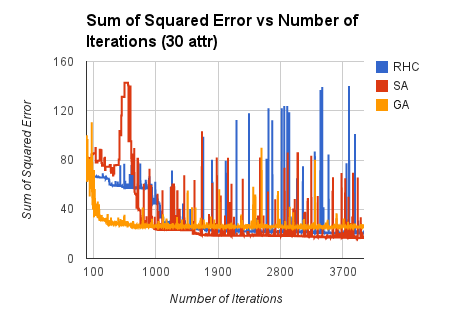
\includegraphics[width=3.5in]{charts/g1_error_vs_iteration_for_rhc_sa_ga_30_attr.png}
  \caption{This graph displays the three algorithms over 4000 iterations for 30 attributes. As can be seen in the graph, 
  the results seem to converge, but suffer from large fluctuations over some iterations due to their random nature. This
  is why a lot of the lines seem to have an abundant number of spikes in their path.}
  \label{fig:g1}
\end{figure}
\begin{table}
    \begin{tabular}{|c|c|c|}
  \hline
        Weight Algorithm    & Accuracy             & Avg. Train Time   \\ \hline
        Backpropagation     & 99.47\%              & 0.021s            \\ 
        RHC                 & 91.92\%              & 197.702s          \\ 
        SA                  & 92.79\%              & 8.661s            \\ 
        GA                  & 89.28\%              & 7.706s            \\
  \hline \end{tabular}
  \caption {Comparison of Algorithm Performance - The average test time for all algorithms was
            nearly identical, averaging 0.003s. Due to this, I felt adding an extra column for
            test time was simply not necessary.} \label{tab:t1l}
  \label{tb:t1}
\end{table}
The general results for 30 attributes over 4,000 iterations can be seen in Figure~\ref{fig:g1}. From the start, I did not
believe that the local random search algorithms would outperform backpropagation, due to the inherent learning from
your mistakes that backpropagation performs. As can be seen in Table~\ref{tb:t1}. This turned out to be a correct
prediction. Backpropagation is the method I used to obtain the weights for my neural network in the first assignment.
\subsection{Analysis}
Over 10 trials, the random nature of these algorithms demonstrated significantly different performance. In my
first iteration, SA for 30 attributes over 4,000 iterations performed terribly (~62\%). My original hypothesis for this
occurring was that the complexity of the problem caused SA to suffer over other methods. However, after observing its
performance over different experiments this hypothesis turned to be false, as my first iteration was clearly an anomaly
that can be observed in the spikes of error for each line that occur in Table~\ref{tb:t1}. Nonetheless, SA had the largest
separation over the 10 trials (lacked precision). The problem can be explained due to the random nature of SA, as it
will succeed at finding a good local maximum, but often not obtain the global maximum. Increasing the number of iterations
for the algorithm after ~1500 iterations had no effect because of the nature of SA, which can sometimes make the wrong 
decision and be incapable of recuperating from said decision. Overall, all of the algorithms converge at approximately
the same number of iterations, although RHC took a significant amount longer to train.
\subsection{Improvements}
\subsubsection{Number of attributes}
\begin{figure}[ht]
  \centering
  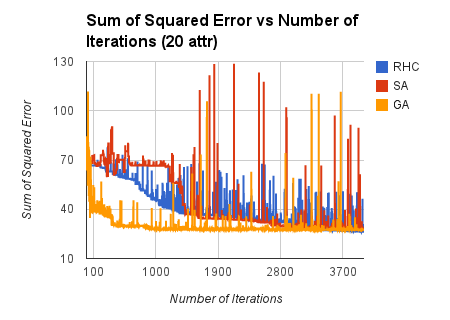
\includegraphics[width=3.5in]{charts/g2_error_vs_iteration_for_rhc_sa_ga_20_attr.png}
  \caption{This graph displays the three algorithms over 4000 iterations for 20 attributes. Although there are significant
  minimum errors in this graph, the idea of a minimum for an random search algorithm's error is insignificant because replication would not be possible (without changing the nature of the algorithm). }
  \label{fig:g2}
\end{figure}
\begin{figure}[ht]
  \centering
  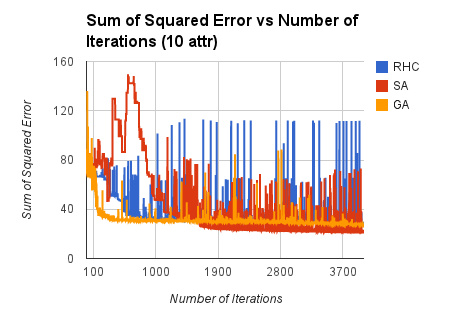
\includegraphics[width=3.5in]{charts/g3_error_vs_iteration_for_rhc_sa_ga_10_attr.png}
  \caption{This graph displays the three algorithms over 4000 iterations for 10 attributes. The results were very similar to 20 and 30 attributes.}
  \label{fig:g3}
\end{figure}
\begin{figure}[ht]
  \centering
  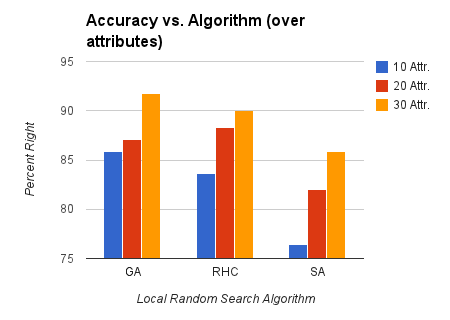
\includegraphics[width=3.5in]{charts/g4_accuracy_vs_algo_rhc_sa_ga.png}
  \caption{This graph compares the average performance of each algorithm over 10 trials. As can be seen, the
  number of attributes does have a positive effect on all of the algorithms.}
  \label{fig:g4}
\end{figure}
My first approach was to improve the algorithm by decreasing the complexity of the dataset. Given its original composition,
which was explained earlier, it was easy to decompose the data into 10 attributes, and 20 attributes. Overall the performance
did not seem to be affected very significantly over the change in algorithm. There is two phenomenons that must be discussed
after analyzing Figure~\ref{fig:g2} and Figure~\ref{fig:g3}. The first concept that must be mentioned is the point of
convergence of the algorithms. They all seem to approach a minimum sum of squared error that can be identified as a really
good local maximum in the space. The second phenomenon is the spikes that SA demonstrate around 1000 iterations. This can be
considered a depiction of the SA algorithm considering a path that in the short term provided worst performance, but in the
long term could lead to a better local maximum.
  
\subsubsection{Simulated Annealing}
In order to analyze simulated annealing in more depth, we conducted an experiment to alter the cooling of the algorithm in order
to see what effect the parameter had on its performance. The previous experiments had all been conducted over a constant cooling
of 0.95. In this experiment we iterated in intervals of 0.05 from 0.05 to 0.95. Cooling must often be tweaked in order to obtain
the best performance for the unique space which the algorithm is searching. The results in Figure~\ref{fig:g5} demonstrate that
the original value we had chosen is actually a good cooling parameter for the experiments. The drops in accuracy further reinforce
the sheer disparity in results that SA may obtain.
\begin{figure}[ht]
  \centering
  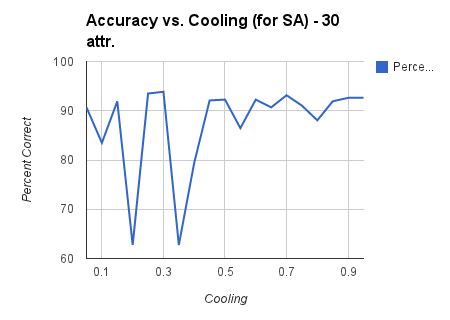
\includegraphics[width=3.5in]{charts/g5_accuracy_vs_cooling_for_sa.png}
  \caption{This demonstrates the effect of altering cooling for simulated annealing. It is important to note that I only ran one
  trial per cooling value, so the drops that can be seen in the graph are most likely due to the error that random algorithms
  presents.}
  \label{fig:g5}
\end{figure}
\subsubsection{Genetic Algorithms}
\begin{figure}[ht]
  \centering
  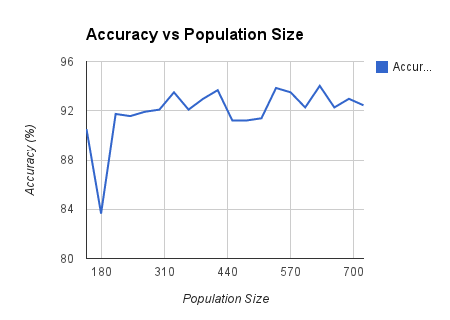
\includegraphics[width=3.5in]{charts/g6_accuracy_vs_pop_for_ga.png}
  \caption{This graph demonstrates that aside from an initial drop in accuracy, a larger population (around 200) has a 
  negligible effect on the accuracy of the algorithm. We take the small changes in accuracy to be strictly due to randomness.}
  \label{fig:g6}
\end{figure}
For GA, we conducted an experiment in order to see if the population size for our evolutionary algorithm had any effect in the
accuracy. Theoretically, I felt that increasing the population size would increase the accuracy prior to reaching (ideally) the
global maximum. However, this did not seem to be the case, as the results seen in Figure~\ref{fig:g6} demonstrate that the
algorithm will not be affected if the population size increases. Reasonably however, if the population size is too small,
it will increase the possibility for error because your ideal solution may no longer be part of the population.

\section{Optimization Problems}
The final part of this analysis focuses on three optimization problems that each individually demonstrate the benefits of SA,
GA, and MIMIC. Our three algorithms will be the Traveling Salesman Problem, the Knapsack Problem, and the Continuous Peaks Problem.
\subsection{Traveling Salesman Problem (TSP)}
\begin{figure}[ht]
  \centering
  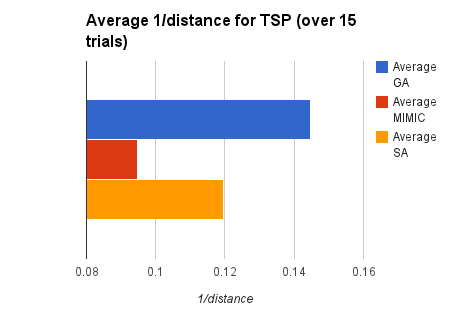
\includegraphics[width=3.5in]{charts/g7_tsp.png}
  \caption{This figure demonstrates the average 1/distance for GA, SA, and MIMIC. The results were averaged over 15 trials, in order
  to obtain an accurate representation of their performance.}
  \label{fig:g7}
\end{figure}
I chose TSP because it benefits heavily off of learning from your iterations to obtain the minimum distance between all of the 
cities. My original hypothesis for this algorithm was that MIMIC would be at the advantage because it learns from previous searches. However, given the complexity of these problems (the sheer magnitude of the possible number of paths), my hypothesis was proven to be flawed. Instead, it demonstrated the advantages of GA in this space. The reason I believe GA outperformed both MIMIC and SA is because the set of populations it defined all were highly probable to contain a small path that was part of the solution. Over several generations and with mutations, the GA was able to combine these small paths into a much more optimal solution which MIMIC and SA were unable to do.

The results can be seen in Figure~\ref{fig:g7}, which demonstrate that GA had the best performance.

\subsection{Knapsack Problem}
\begin{figure}[ht]
  \centering
  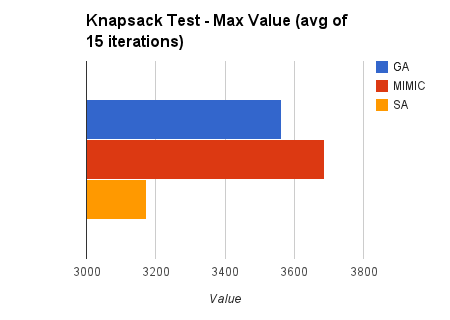
\includegraphics[width=3.5in]{charts/g8_knapsack.png}
  \caption{This figure demonstrates the average maximum value obtained for GA, SA, and MIMIC. On average, MIMIC scored 3686, GA 
  scored 3562, and SA scored 3117. }
  \label{fig:g8}
\end{figure}
I decided to analyze the Knapsack Problem because it is a trivial problem to get a decent result, but a much more complex problem if
you need the best result. My original hypothesis was that this would demonstrate the advantages of MIMIC due to its capabilities to
learn from searching the space. This hypothesis was in fact proven true, as can be seen in Figure~\ref{fig:g8}. This problem is vital
in demonstrating the weaknesses of SA which perform decently when the outcome need not be close to perfect. In this case, MIMIC
outperforms both of them because GA and SA are unable to converge to a better solution, which can be defined as a larger total value
in the sack.  The standard genetic algorithm used in ABAGAIL actually does a decent job at defining a population which allows it to
obtain a decent result. 
\subsection{Continuous Peaks Problem}
\begin{figure}[ht]
  \centering
  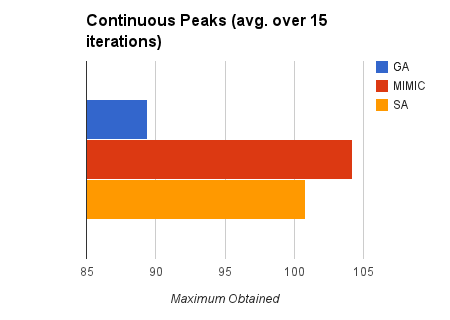
\includegraphics[width=3.5in]{charts/g9_cp.png}
  \caption{This figure demonstrates the average maximum values obtained for the Continuous Peaks problem. It demonstrates the
  advantages of MIMIC and SA in solving the problem. }
  \label{fig:g9}
\end{figure}
\begin{figure}[ht]
  \centering
  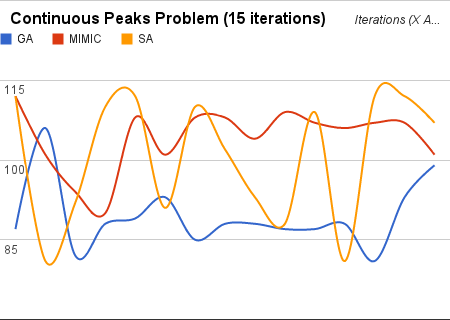
\includegraphics[width=3.5in]{charts/g10_cp.png}
  \caption{This figure was smoothed in order to better illustrate the performance of SA. These 15 trials demonstrate the 
  consistency and precision of the algorithms when run over multiple iterations. The maximum value obtained over all the
  algorithms and all the trials was 112, which was obtained once by MIMIC, and 4 times by SA.}
  \label{fig:g10}
\end{figure}
The last problem I decided to focus on was Continuous Peaks because I felt like it further demonstrates the advantages of
MIMIC, but also was ideal in illustrating why SA was introduced. My original hypothesis was that MIMIC would outperform the
other algorithms, but SA would still peform significantly better than the GA, and this in fact proved to be the case. As can
be seen in Figure~\ref{fig:g9}, MIMIC is able to correctly search the space for an ideal maximum, and the trials demonstrate
that it is a significant amount more consistent in obtaining these results. After investigating the consistency, I graphed the
15 trials in order to provide more insight into the volatility of SA. Equally so, this demonstrates an advantage of MIMIC,
it is the most accurate because of its precision over 15 trials.

As can be seen in Figure ~\ref{fig:g10}, the best performance of SA is actually equal to that of MIMIC. However, the same
can be said about the worst peformance, wherein SA performs equally as bad as GA in other trials. This demonstrates the overall
volatility of SA, and the more consistent nature of MIMIC. In this case, on average, it can be said that you will obtain a better
performance from MIMIC because it fluctuates a significant amount less.
\section{Conclusion}
In this paper I examined the use of three randomized optimization algorithms in order to obtain weights for a neural network,
and then compared them to a previous result from ~\cite{Castro:2013} on the Wisconsin Breast Cancer Diagnostic dataset which
used backpropagation to obtain its weights. In this scenario, backpropagation still outperformed RHC, SA, and GA, who all
obtained very similar performance. I then further examined SA, GA and MIMIC with respect to optimization problems that would
demonstrate the advantages of each approach. This entire analysis expanded my understanding of optimization algorithms, and
their use in machine learning, and real world problem solving.
\section{Future Work}
I would further like to examine the potential use of different datasets with independent attributes in order to see how the
performance of each algorithm changes with more or less attributes (in our case the dataset had dependent attributes). Further,
i'd like to analyze other optimization problems that may allow me to learn novel concepts about the algorithms that were presented,
in order to fully understand their advantages and disadvantages. Lastly, I'd like to tweak the parameters for each specific 
algorithm in order to see if it has an effect on their performance.
\section*{Acknowledgements}
First, I'd like to acknowldege~\cite{Frank+Asuncion:2010} and the 
University of Wisconsin as well for the Wisconsin Breast Cancer 
(Diagnostic) dataset. Further, I would like to acknowledge everyone 
involved in the construction of the ABAGAIL Java library, which was 
essential for running the algorithms in this project. Lastly, i'd
like to recognize the fact that the backpropagation algorithm for my
neural network comparison was obtained using Weka~\cite{Hall_weka:2010}.
\bibliographystyle{acmsiggraph}
\bibliography{machine_learning_p2}
\end{document}
